


\chapter{Minimalist Automated Prover\label{ch:prover}}
%-----------------------------------------------------------------------------
At the core of any mechanical verification system is an automated theorem prover responsible for discharging VCs.  By definition, it is the last word on whether or not a particular technique is yielding more or less easily-proved VCs.  As a result of this, most practical systems have focussed on incorporating the latest and greatest provers into their retinue to piggyback on the breakthroughs at the bleeding edge of proving and artificial intelligence and thus increase provability.

While we are happy to support the latest and greatest suite of provers, we hypothesize that in many cases \emph{flexibility} may trump raw performance with respect to mechanically verifying well-engineered software by encouraging good specification and mathematical engineering that captures the programmer's intuition rather than compromising to work within the framework of a target prover.

In order to experiment with this hypothesis and identify those prover capabilities and performance tunings required to verify well-engineered software, we set out to create a \emph{minimalist automated prover}, starting with only the bare essential capabilities and expanding only when a significant number of VCs appeared that could not be addressed with the prover as it stood.  The result of this effort was RESOLVE's integrated rewrite prover.  As we've refined our design, it has become a platform for prover experimentation within the group and we intend to use it as the yardstick against which to measure our success using our new mathematical system to verify components.


%-----------------------------------------------------------------------------
\section{Initial Observations and the Version 1 Prover}
%-----------------------------------------------------------------------------

In practical verification systems to date, specifications are often quite complicated, even for simple operations.  These specifications derive 


In \cite{smith10}, we present our architecture for an extensible platform for minimalistic prover experimentation.  The implementation of this prover is in a working form and has been used for several years as part of the RESOLVE toolchain, incuding as part of our education effort centered around the RESOLVE integrated web development environment\cite{chuckThesis}.  This prover has been used in support of a number of our verification publications, including \cite{Sit11} and \cite{smithMinimalist}.  We see the results of a successful verification from the web interface in Figure \ref{fig:successfulverification}.  This is a verification of a realization of the \texttt{Flip()} operation introduced in Section \ref{sec:resolveBackground}.  Enhancement realizations often involve a small number of mathematical types (in this case, almost entirely Strings) and are therefore more straightforward to verify.  Data structure realizations, on the other hand, often have to map from one representation to another, introducing many related types.  As a result, while we can prove them by hand, the mechanical verification of data structures is consigned to Work to be Completed.

\begin{figure}
  \centering
    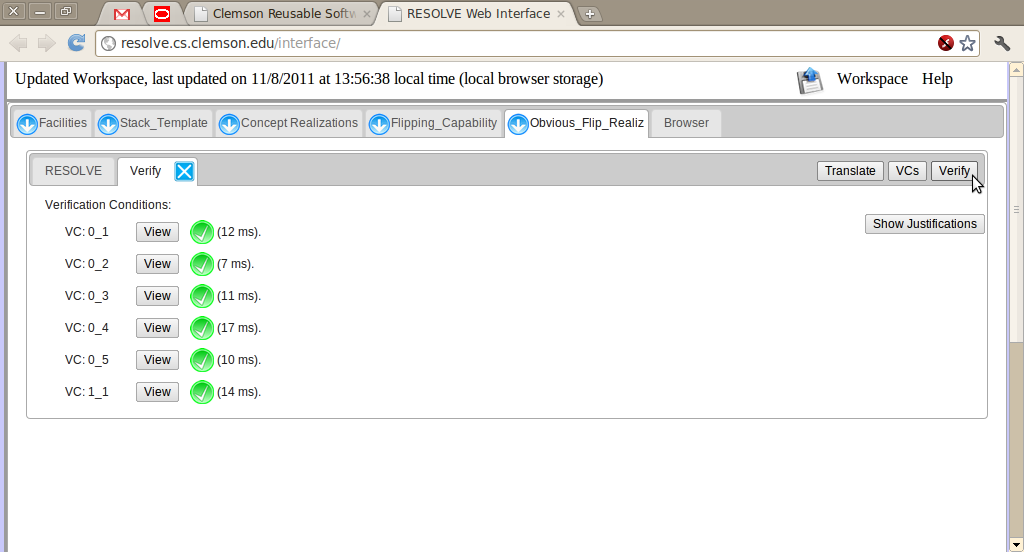
\includegraphics[width=\textwidth]{successfulverification}
  \caption{Our Minimalist Prover at Work\label{fig:successfulverification}}
\end{figure}

As part of our experimentation to-date, we have utilized the extensible plug-in architecture of the prover to add a number of capabilities.  These have included heuristics to make intelligent theorem choices based on the VC at hand, a graphical front-end that permits the user to guide the prover, and a number of preprocessing options to simplify and normalize incoming VCs.  In \cite{smithMinimalist} we perform a comparison of proof complexity (in terms of number of proof steps, including backtracks, taken before reaching a complete proof) based on a simple component using a number of different feature configurations.  This exploration was very illuminating as to which features gave good results.

%-----------------------------------------------------------------------------
\subsubsection{Work To Be Completed}
%-----------------------------------------------------------------------------
With the harness already in working order, the most important addition is that of facilities for mechanically characterizing VCs according to a number of different mechanisms.  Our current depth-first search is more efficient than a breadth-first search, but means that we do not necessarily find the \emph{shortest} proof.  Work is needed to permit a breadth first option when we're willing to trade some efficiency for a more precise metrics.  In addition, we imagine some metrics will be related to the theorems used and the current prover output takes the form of a plain-text ASCII dump, which is not ideal for processing.  A better solution must be engineered so that proofs can be compared and processed mechanically.

Additionally, we would like to expand our efforts to collect data on different prover feature configurations by applying this analysis to a broader range of components.  As mentioned in the Work Completed section, we are eager to expand mechanical verification from enhancement realizations to data structure realizations.  This process will include the explorations of features that have yet to be identified and may be included upon discovering their usefulness for practical VCs.  As an example of a capability we have identified but have yet to implement, we consider a snippet from a realization of a \texttt{Merge\_Sort()} enhancement for queues.  As part of a loop invariant we state:

\texttt{Is\_Permutation(\#Q o \#R, Merger o <Q\_Min> o Q o R)}

Clearly, in the context of a permutation, the concatenation operator is commutative.  Unfortunately, any straightforward commutativity theorem requires us to play a complicated shell game to rearrange arbitrary chains of concatenation.  We could use a torrent of theorems to try and cover all cases, but we suspect that at that point, we have followed minimalism to a ridiculous extreme.  We would like, instead, to permit such context-sensitive properties to be stated in a general way, after which a better internal prover representation than a tree could be chosen to better reflect the properties of the conjunct.

We would also like to experiment with minimalistic proving algorithms.  For example, in addition to the back-tracking, depth- or breadth-first search algorithm we establish in \cite{smith10}, we could imagine that we instead start with our set of antecedents and our set of consequents, then transitively build up a larger and larger set of known antecedents as we simultaneously build up a set of possible justifications for each conjunct of the consequents, dispatch a conjunct whenever its justification set intersects the antecedent set. 

Finally, the prover will need to be adapted to work with the new mathematical type-system, though this modification should be straight-forward since complex reasoning about types is unnecessary in the prover, which need only be able to answer the questions ``What is the type of this expression?'' and ``Does an expression of this type bind to this free variable?''  The former question ought to be answered before the prover is ever invoked, while the latter should be a straightforward library call to the symbol table.

